\newcommand{\mysection}[1]{\vspace{-.00cm}\section{#1}\vspace{-.00cm}}
\newcommand{\mysubsection}[1]{\vspace{-.00cm}\subsection{#1}\vspace{-.00cm}}
\newcommand{\mysubsubsection}[1]{\vspace{-.00cm}\subsubsection{#1}\vspace{-.00cm}}

%\documentclass{acm_proc_article-sp}
\documentclass[12pt,twocolumn]{article}

\usepackage{multirow}
\usepackage{times}
\usepackage[scaled=0.92]{helvet}
\usepackage[T1]{fontenc}
\usepackage{enumerate}
\usepackage{textcomp}
\usepackage{graphicx}
\usepackage[pdftex]{hyperref}
\usepackage{url}
\usepackage{mathptmx}
\usepackage{bbm}
\usepackage{dsfont}
\usepackage{subfig}
\usepackage[noadjust]{cite}
\usepackage{array}
\usepackage{fancyvrb}
\usepackage{listings}
\usepackage[super]{nth}

\begin{document}
\title{A Look at Artificial Neural Networks}
\date{}

%\numberofauthors{1}
%\author{
%\alignauthor Aaron Cahn\\
%\affaddr{University of Wisconsin-Madison}\\
%\email{cahn@cs.wisc.edu}
%}


\author{
Aaron Cahn\\
University of Wisconsin-Madison\\
cahn@cs.wisc.edu
}


\maketitle
\begin{abstract}
In this study we implement a general artificial neural network framework.
Our framework allows us to construct neural networks with arbitrary input, hidden, and output units as well as an arbitrary number of hidden layers.
The user is also able to specify the learn rate, number of epochs to train the neural network, and whether to do cross validated training with n folds.
This framework allows us to explore the performance and accuracy trade offs of varying the neural network parameters.
For this study, we utilize the Wisconsin Breast Cancer data set~\cite{wolberg1990multisurface} to motivate the necessity of parameter space exploration.
We also compare the performance and accuracy of training a single neural network to that of training an ensemble of neural networks.
We show <list some results/generalizations>.

\end{abstract}

\section{Introduction} \label{sec:intro} Artificial neural networks were originally inspired by the complex web of neurons that create the human brain.
The core of a neural network is the perceptron, which is a simple representation of a neuron consisting of an activation function.
The activation function is responsible for producing the output of the perceptron.
Perceptrons are linked together in layers to form what is generally known as a multi-layer neural network.
Historically, neural networks consist of an input layer, a single hidden layer, and an output layer.
All layers are completely connected to the next layer and edge weights from layer \(i\) to layer \(i+1\) are trained by an algorithm known as back propagation.
Because of this, a neural network with a hidden layers can represent arbitrary functions.

When a neural network contains more than a single layer, it is often referred to as a deep network.
However, there is debate over whether this criteria alone constitutes a deep network.
Generally, training a deep network through backpropagation alone is insufficient because of the large number of local minimum that exist on the complex error surface.
Therefore, different techniques, which incrementally train a layer of weights at a time, are needed for deep networks.

Neural networks, and more specifically the edge weights from layer to layer, can easily be represented by matrices.
This representation lends itself to fast, parallel computations.
As a result, neural networks are extremely popular for tasks that require a complex representation space.
Many groups have used neural networks for modeling complex systems, performing image recognition tasks, and performing autonomous tasks such as flying a helicopter. {\bf citation}

In this paper we focus on neural networks with one and two hidden layers.
Attempting to utilize more than two hidden layers trained using standard backpropagation does not improve accuracy over the data sets we use.
Extending the neural network framework to include a deep training function is left to future work as we were unable to implement it before the deadline.

Our paper attempts to shed light on the trade offs a researcher can make between performance and computation cost.
We motivate this by exploring the parameter space of our neural network framework and demonstrating the accuracy under different network configurations.
We also explore building an ensemble of neural networks on top of our framework.
We make the following contributions: <list contributions>

The rest of this paper is organized as follows.
Section~\ref{sec:design} explains the design and implementation choices of our framework.
Section~\ref{sec:methodology} explains the data sets we use for experimentation and the experiments we ran.
Section~\ref{sec:results} reports the results from the experiments we ran on our framework.
Section~\ref{sec:summary} concludes.

\section{Design and Implementation} \label{sec:design} The artificial neural network was implemented in Python.
It consists of a single class which takes as arguments (i) the number of input units (ii) a list containing the number hidden units to create at each hidden layer (where the length of the list defines the number of hidden layers to create (iii) the number of output units (iv) the learn rate and (v) the number of epochs to train the neural network for.
The neural network unit activations, errors, and weights are represented simply as matrices.
This allows all computations to be down in a fast and efficient manner and makes the neural network implementation very comphrensible.
The neural network class exports functions to (i) feed a single instance through the network (ii) run backpropagation (iii) train on a set of data (iv) test a set of data and (v) a set of functions to print weights, errors, and activations for debugging from the command line.
 


\section{Methodology} \label{sec:methodology} METHODOLOGY CHECKLIST:\\
1. Explain the data set and data set scrubbing\\
2. Explain experimental setup and experiments run\\
3. Explain the hypothesis and general experiment framework (how this works for any data set)

\section{Results} \label{sec:results} %\begin{table*}
%
%    \begin{center}
%      \title{Accuracy while varying the number hidden layer units}
%      \begin{tabular}{|l|l|l|l|l|l|l|l|l|l|l|}
%        \hline
%        Layers & 1     & 2     & 3     & 4     & 5     & 6     & 7     & 8     & 9     & 10    \\ \hline
%        0               & 65.01 & 71.18 & 71.47 & 68.10 & 77.61 & 71.24 & 77.86 & 80.90 & 80.90 & 83.98 \\ \hline
%        1               & 65.01 & 65.01 & 65.01 & 68.40 & 72.51 & 70.01 & 68.20 & 70.58 & 70.95 & 77.50 \\ \hline
%        2               & 65.01 & 65.01 & 67.90 & 82.71 & 74.08 & 89.73 & 87.58 & 88.27 & 91.94 & 91.05 \\ \hline
%        3               & 65.01 & 65.01 & 73.93 & 84.18 & 92.96 & 89.43 & 91.93 & 91.93 & 91.79 & 91.05 \\ \hline
%        4               & 65.01 & 68.10 & 76.72 & 85.17 & 89.88 & 92.81 & 92.81 & 93.10 & 92.81 & 92.96 \\ \hline
%        5               & 65.01 & 65.01 & 70.99 & 91.19 & 87.80 & 90.20 & 93.69 & 92.96 & 93.84 & 93.98 \\ \hline
%        6               & 65.01 & 65.01 & 70.85 & 88.50 & 91.49 & 93.98 & 92.67 & 93.99 & 93.98 & 94.28 \\ \hline
%        7               & 65.01 & 65.01 & 77.02 & 85.94 & 94.28 & 94.86 & 94.71 & 94.72 & 95.01 & 94.28 \\ \hline
%        8               & 65.01 & 65.01 & 68.54 & 83.50 & 91.82 & 91.67 & 94.86 & {\bf 95.60} & 94.87 & 95.15 \\ \hline
%        9               & 65.01 & 68.20 & 74.18 & 92.06 & 94.86 & 92.22 & 95.30 & 94.72 & 95.45 & 95.16 \\ \hline
%        10              & 65.01 & 65.01 & 73.74 & 80.84 & 91.92 & 95.30 & 95.59 & 95.59 & 95.30 & 95.30 \\ \hline
%      \end{tabular}
%    \end{center}
%    \label{tab:breast}
%    \caption {Accuracy for neural networks with one and two hidden layers. Entry \(i,j\) represents a neural network with \(j\) units in the first hidden layer and \(i\) units in the second hidden layer ({\em i.e.,} row 0 represents neural networks with only one hidden layer). The bold entry represents max accuracy.}
%
%\end{table*}

\begin{figure*}[t]
  \title{Accuracy at Various Hidden Unit/Layer Combinations}
\centering
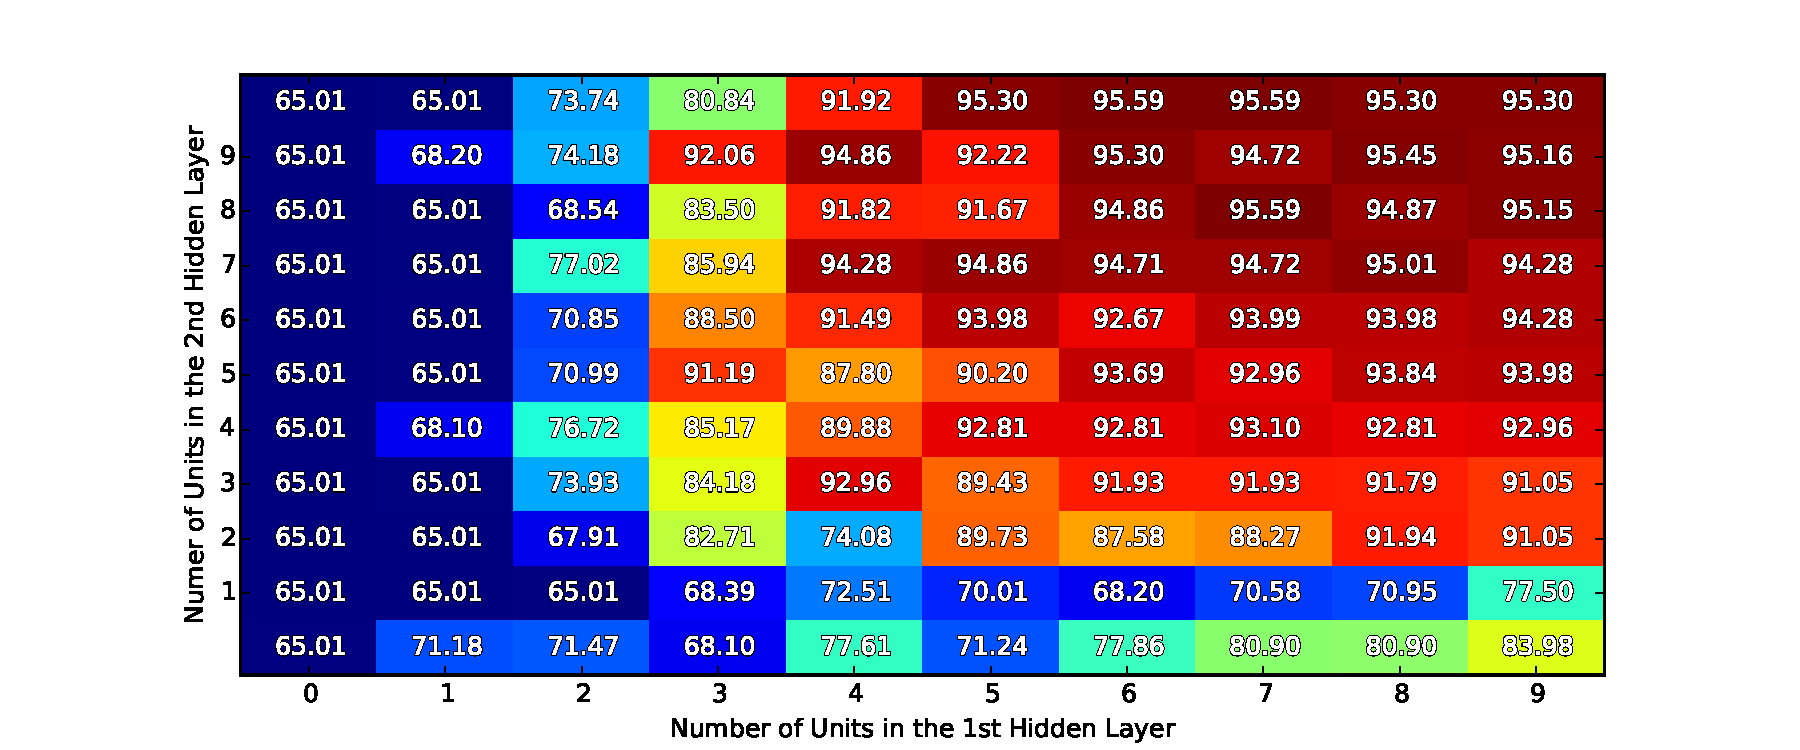
\includegraphics[width=\textwidth]{figs/wbcd_table}
\caption {Accuracy for neural networks with one and two hidden layers. Entry \(i,j\) represents a neural network with \(j\) units in the first hidden layer and \(i\) units in the second hidden layer ({\em i.e.,} row 0 represents neural networks with only one hidden layer). The bold entry represents max accuracy.}

\label{fig:wbcd_table}

\end{figure*}


Plots we have data for:\\
1. average accuracy for 1 hidden layer hidden units vary from 1-10 using 10 fold cross validation, epoch = 10\\
2. average accuracy for 2 hidden layer hidden units vary from 1-10 using 10 fold cross validation, epoch = 100\\
(1 and 2 will be combined into a single table, wbcd data)\\
3. average accuracy for 1 hidden layer hidden units vary from 1-120, epoch = 1000\\
4. average accraucy for 2 hidden layer hidden units vary from 1-120, epoch = 1000\\
(3 and 4 will combine into a single table, face data)\\

TODO: Add the results\\
5. Ensemble of neural networks using the best combination of parameters from 1 and 2 (plot varying the number of neural nets)\\
6. Ensemble of neural networks using the best combination of parameters from 3 and 4 (plot varying the number of neural nets)\\
 














\section{Summary and Conclusions} \label{sec:summary} SUMMARY CHECKLIST:\\
1. Take synthesized result and generalize into general rules about the need to search parameter spaces exhaustively\\
2. Talk about the consideration that need to made for choosing between certain tradoffs
3. Conclude


\bibliographystyle{plain}
\bibliography{paper}

\end{document}
